% Options for packages loaded elsewhere
\PassOptionsToPackage{unicode}{hyperref}
\PassOptionsToPackage{hyphens}{url}
%
\documentclass[
  ignorenonframetext,
  aspectratio=43,
]{beamer}
\usepackage{pgfpages}
\setbeamertemplate{caption}[numbered]
\setbeamertemplate{caption label separator}{: }
\setbeamercolor{caption name}{fg=normal text.fg}
\beamertemplatenavigationsymbolshorizontal
% Prevent slide breaks in the middle of a paragraph
\widowpenalties 1 10000
\raggedbottom
\setbeamertemplate{part page}{
  \centering
  \begin{beamercolorbox}[sep=16pt,center]{part title}
    \usebeamerfont{part title}\insertpart\par
  \end{beamercolorbox}
}
\setbeamertemplate{section page}{
  \centering
  \begin{beamercolorbox}[sep=12pt,center]{part title}
    \usebeamerfont{section title}\insertsection\par
  \end{beamercolorbox}
}
\setbeamertemplate{subsection page}{
  \centering
  \begin{beamercolorbox}[sep=8pt,center]{part title}
    \usebeamerfont{subsection title}\insertsubsection\par
  \end{beamercolorbox}
}
\AtBeginPart{
  \frame{\partpage}
}
\AtBeginSection{
  \ifbibliography
  \else
    \frame{\sectionpage}
  \fi
}
\AtBeginSubsection{
  \frame{\subsectionpage}
}

\usepackage{amsmath,amssymb}
\usepackage{lmodern}
\usepackage{iftex}
\ifPDFTeX
  \usepackage[T1]{fontenc}
  \usepackage[utf8]{inputenc}
  \usepackage{textcomp} % provide euro and other symbols
\else % if luatex or xetex
  \usepackage{unicode-math}
  \defaultfontfeatures{Scale=MatchLowercase}
  \defaultfontfeatures[\rmfamily]{Ligatures=TeX,Scale=1}
\fi
\usetheme[]{default}
\usecolortheme{default}
% Use upquote if available, for straight quotes in verbatim environments
\IfFileExists{upquote.sty}{\usepackage{upquote}}{}
\IfFileExists{microtype.sty}{% use microtype if available
  \usepackage[]{microtype}
  \UseMicrotypeSet[protrusion]{basicmath} % disable protrusion for tt fonts
}{}
\makeatletter
\@ifundefined{KOMAClassName}{% if non-KOMA class
  \IfFileExists{parskip.sty}{%
    \usepackage{parskip}
  }{% else
    \setlength{\parindent}{0pt}
    \setlength{\parskip}{6pt plus 2pt minus 1pt}}
}{% if KOMA class
  \KOMAoptions{parskip=half}}
\makeatother
\usepackage{xcolor}
\newif\ifbibliography
\setlength{\emergencystretch}{3em} % prevent overfull lines
\setcounter{secnumdepth}{-\maxdimen} % remove section numbering


\providecommand{\tightlist}{%
  \setlength{\itemsep}{0pt}\setlength{\parskip}{0pt}}\usepackage{longtable,booktabs,array}
\usepackage{calc} % for calculating minipage widths
\usepackage{caption}
% Make caption package work with longtable
\makeatletter
\def\fnum@table{\tablename~\thetable}
\makeatother
\usepackage{graphicx}
\makeatletter
\def\maxwidth{\ifdim\Gin@nat@width>\linewidth\linewidth\else\Gin@nat@width\fi}
\def\maxheight{\ifdim\Gin@nat@height>\textheight\textheight\else\Gin@nat@height\fi}
\makeatother
% Scale images if necessary, so that they will not overflow the page
% margins by default, and it is still possible to overwrite the defaults
% using explicit options in \includegraphics[width, height, ...]{}
\setkeys{Gin}{width=\maxwidth,height=\maxheight,keepaspectratio}
% Set default figure placement to htbp
\makeatletter
\def\fps@figure{htbp}
\makeatother

\usepackage{ragged2e}
\usepackage{etoolbox}

\apptocmd{\frame}{}{\justifying}{} 

\setbeamertemplate{enumerate items}[default]
\setbeamertemplate{itemize items}[circle]
\setbeamersize{text margin left=2.25em, text margin right=2.25em}

\let\OLDitemize\itemize
\renewcommand\itemize{
    \OLDitemize\addtolength{\itemsep}{3pt plus 1pt minus 1pt}
}
\let\OLDenumerate\enumerate
\renewcommand\enumerate{
    \OLDenumerate\addtolength{\itemsep}{3pt plus 1pt minus 1pt}
}

\usepackage{orcidlink}
\usepackage{amsmath}
\DeclareMathOperator*{\argmax}{argmax}

\makeatletter
\def\@listii{\leftmargin\leftmarginii
              \topsep    1ex
              \parsep    0\p@   \@plus\p@
              \itemsep   \parsep}
\makeatother

\usepackage{lipsum}

\let\olditem\item
\renewcommand\item{\olditem\justifying}

\definecolor{blue}{RGB}{0,114,178}
\definecolor{red}{RGB}{213,94,0}
\definecolor{yellow}{RGB}{240,228,66}
\definecolor{green}{RGB}{0,158,115}

\definecolor{MyBackground}{RGB}{255,253,218}

\setbeamercolor{section in toc}{fg=blue}
\setbeamercolor{subsection in toc}{fg=red}

\setbeamercolor{frametitle}{fg=blue}
\setbeamercolor{title}{fg=blue}

\setbeamertemplate{footline}[frame number]
\setbeamertemplate{navigation symbols}{} 
\setbeamertemplate{itemize items}{-}

\setbeamercolor{itemize item}{fg=blue}
\setbeamercolor{itemize subitem}{fg=blue}
\setbeamercolor{enumerate item}{fg=blue}
\setbeamercolor{enumerate subitem}{fg=blue}
\setbeamercolor{button}{bg=MyBackground,fg=blue}

\newcounter{daggerfootnote}
\newcommand*{\daggerfootnote}[1]{%
    \setcounter{daggerfootnote}{\value{footnote}}%
    \renewcommand*{\thefootnote}{\fnsymbol{footnote}}%
    \footnote[2]{#1}%
    \setcounter{footnote}{\value{daggerfootnote}}%
    \renewcommand*{\thefootnote}{\arabic{footnote}}%
}

\AtBeginSection{
    \begingroup
    \setbeamercolor{background canvas}{bg=yellow}
    \begin{frame}
        \begin{centering}
            \usebeamerfont{section title}\huge\color{black}\insertsection\par
        \end{centering}
    \end{frame}
    \endgroup
}
\makeatletter
\makeatother
\makeatletter
\makeatother
\makeatletter
\@ifpackageloaded{caption}{}{\usepackage{caption}}
\AtBeginDocument{%
\ifdefined\contentsname
  \renewcommand*\contentsname{Table of contents}
\else
  \newcommand\contentsname{Table of contents}
\fi
\ifdefined\listfigurename
  \renewcommand*\listfigurename{List of Figures}
\else
  \newcommand\listfigurename{List of Figures}
\fi
\ifdefined\listtablename
  \renewcommand*\listtablename{List of Tables}
\else
  \newcommand\listtablename{List of Tables}
\fi
\ifdefined\figurename
  \renewcommand*\figurename{Figure}
\else
  \newcommand\figurename{Figure}
\fi
\ifdefined\tablename
  \renewcommand*\tablename{Table}
\else
  \newcommand\tablename{Table}
\fi
}
\@ifpackageloaded{float}{}{\usepackage{float}}
\floatstyle{ruled}
\@ifundefined{c@chapter}{\newfloat{codelisting}{h}{lop}}{\newfloat{codelisting}{h}{lop}[chapter]}
\floatname{codelisting}{Listing}
\newcommand*\listoflistings{\listof{codelisting}{List of Listings}}
\makeatother
\makeatletter
\@ifpackageloaded{caption}{}{\usepackage{caption}}
\@ifpackageloaded{subcaption}{}{\usepackage{subcaption}}
\makeatother
\makeatletter
\@ifpackageloaded{tcolorbox}{}{\usepackage[many]{tcolorbox}}
\makeatother
\makeatletter
\@ifundefined{shadecolor}{\definecolor{shadecolor}{rgb}{.97, .97, .97}}
\makeatother
\makeatletter
\makeatother
\ifLuaTeX
  \usepackage{selnolig}  % disable illegal ligatures
\fi
\IfFileExists{bookmark.sty}{\usepackage{bookmark}}{\usepackage{hyperref}}
\IfFileExists{xurl.sty}{\usepackage{xurl}}{} % add URL line breaks if available
\urlstyle{same} % disable monospaced font for URLs
\hypersetup{
  pdftitle={Seminar 8},
  pdfauthor={Gabriel E. Cabrera Guzmán},
  hidelinks,
  pdfcreator={LaTeX via pandoc}}

\title[Seminar 8]{Seminar
8\daggerfootnote{\texttt{gabriel.cabreraguzman@postgrad.manchester.ac.uk}}}
\subtitle{Statistics 5 (Correlation and Regression) Solutions}
\author[Gabriel E. Cabrera Guzmán]{
    {Gabriel E. Cabrera
Guzmán\textsuperscript{\normalsize\orcidlink{0000-0000-0000-0000}}} \medskip
}
\date{December 7, 2025}
\institute[]{
    The University of Manchester\\
Alliance Manchester Business School \bigskip
}

\definecolor{quarto-callout-note-color}{RGB}{0,114,178}
\definecolor{quarto-callout-note-color-frame}{RGB}{0,114,178}
\definecolor{quarto-callout-warning-color}{RGB}{213,94,0}
\definecolor{quarto-callout-warning-color-frame}{RGB}{213,94,0}
\begin{document}
\frame{\titlepage}
\ifdefined\Shaded\renewenvironment{Shaded}{\begin{tcolorbox}[interior hidden, enhanced, borderline west={3pt}{0pt}{shadecolor}, frame hidden, breakable, boxrule=0pt, sharp corners]}{\end{tcolorbox}}\fi

\begin{frame}{Exercise 1}
\protect\hypertarget{exercise-1}{}
Suppose two cryptocurrencies' monthly returns have a correlation
coefficient of 0.33 based on observations from the previous 24 months.

\pause

\begin{enumerate}
\item
  Test the claim that the correlation is greater than zero using a 5\%
  level of significance.

  \pause

  The correlation coefficient is 0.33 and the sample size is 24.
  Therefore, we have

  \pause

  \[
   t=r\sqrt{\frac{{n-2}}{1-r^2}} = 0.33\sqrt{\frac{24-2}{1-0.33^2}} \approx 1.64
   \]

  \pause

  \[
   \begin{aligned}
   H_0 &: \rho = 0 \\
   H_1 &: \rho > 0
   \end{aligned}
   \]
\end{enumerate}
\end{frame}

\begin{frame}{Exercise 1 (Cont'd)}
\protect\hypertarget{exercise-1-contd}{}
\pause

The significance level is \(\alpha=5\%\). To find the critical value for
rejecting the null at this significance level, we look for the
probability of 0.05 in the \textbf{Student's t-distribution} table with
a degree of freedom \(df=n-2=24-2=22\). For a \textbf{right-tailed
test}, we look for the value t such that the probability to its
\textbf{right} is 0.05. From the table, we find that
\(Pr(T <1.72) = 0.95\). Therefore, the critical value for a right-tailed
test at the 5\% significance level is 1.72. Since the t-test statistic
(1.64) is \emph{less} than the critical value (1.72), we fail to reject
the null hypothesis at a 5\% level of significance.
\end{frame}

\begin{frame}{Exercise 1 (Cont'd)}
\protect\hypertarget{exercise-1-contd-1}{}
\pause

\vspace{15pt}

\begin{figure}

{\centering 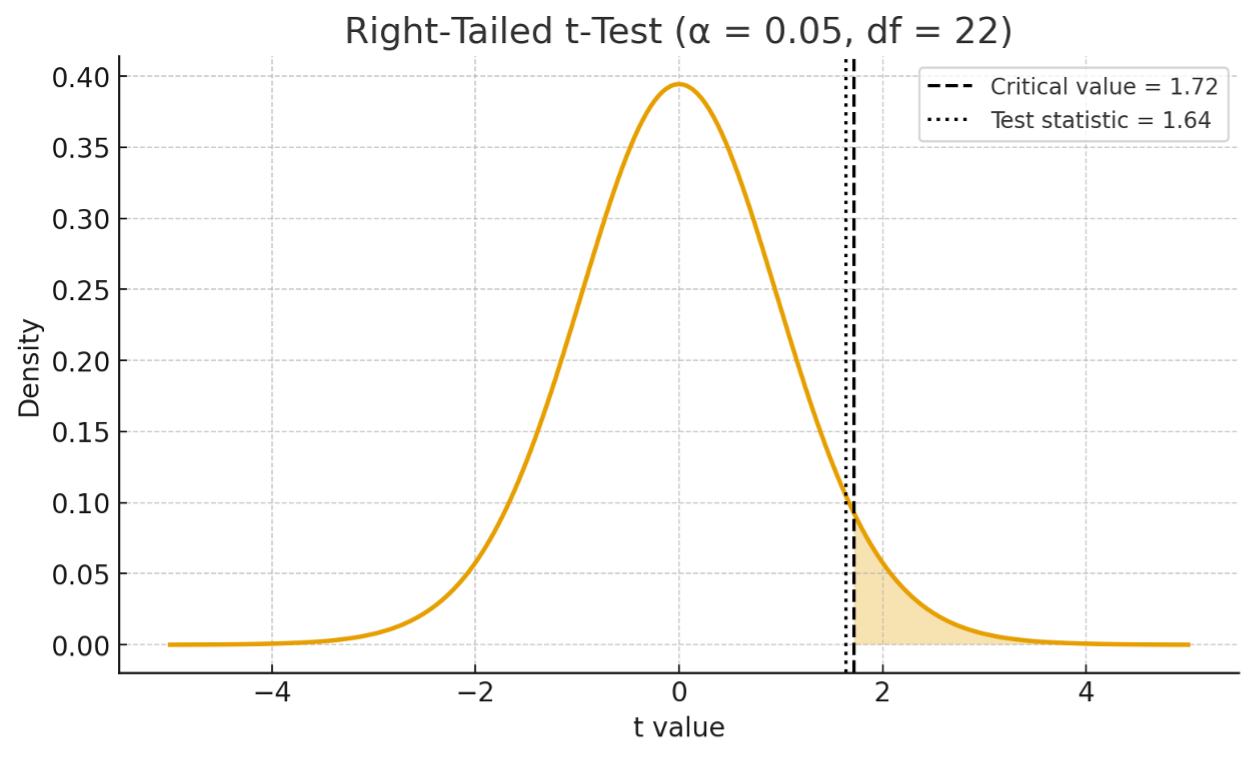
\includegraphics[width=0.95\textwidth,height=\textheight]{Fig/q1_a.png}

}

\end{figure}
\end{frame}

\begin{frame}{Exercise 1 (Cont'd)}
\protect\hypertarget{exercise-1-contd-2}{}
\begin{enumerate}
\setcounter{enumi}{1}
\item
  Test the claim that the correlation is less than zero using a 5\%
  level of significance.\vspace{-5pt}

  \pause

  \[
   \begin{aligned}
   H_0 &: \rho = 0 \\
   H_1 &: \rho < 0
   \end{aligned}
   \]

  \pause

  The significance level is \(\alpha=5\%\). To find the critical value
  for rejecting the null at this significance level, we look for the
  probability of 0.05 in the \textbf{Student's t-distribution} table
  with a degree of freedom \(df=n-2=24-2=22\). For a \textbf{left-tailed
  test}, we look for the value t such that the probability to its
  \textbf{left} is 0.05. From the table, we find that
  \(Pr(T>-1.72)= 0.95\). Therefore, the critical value for a left-tailed
  test at the 5\% significance level is -1.72. Since the t-test
  statistic (1.64) is \emph{greater} than the critical value (-1.72), we
  fail to reject the null hypothesis at a 5\% level of significance.
\end{enumerate}
\end{frame}

\begin{frame}{Exercise 1 (Cont'd)}
\protect\hypertarget{exercise-1-contd-3}{}
\pause

\vspace{15pt}

\begin{figure}

{\centering 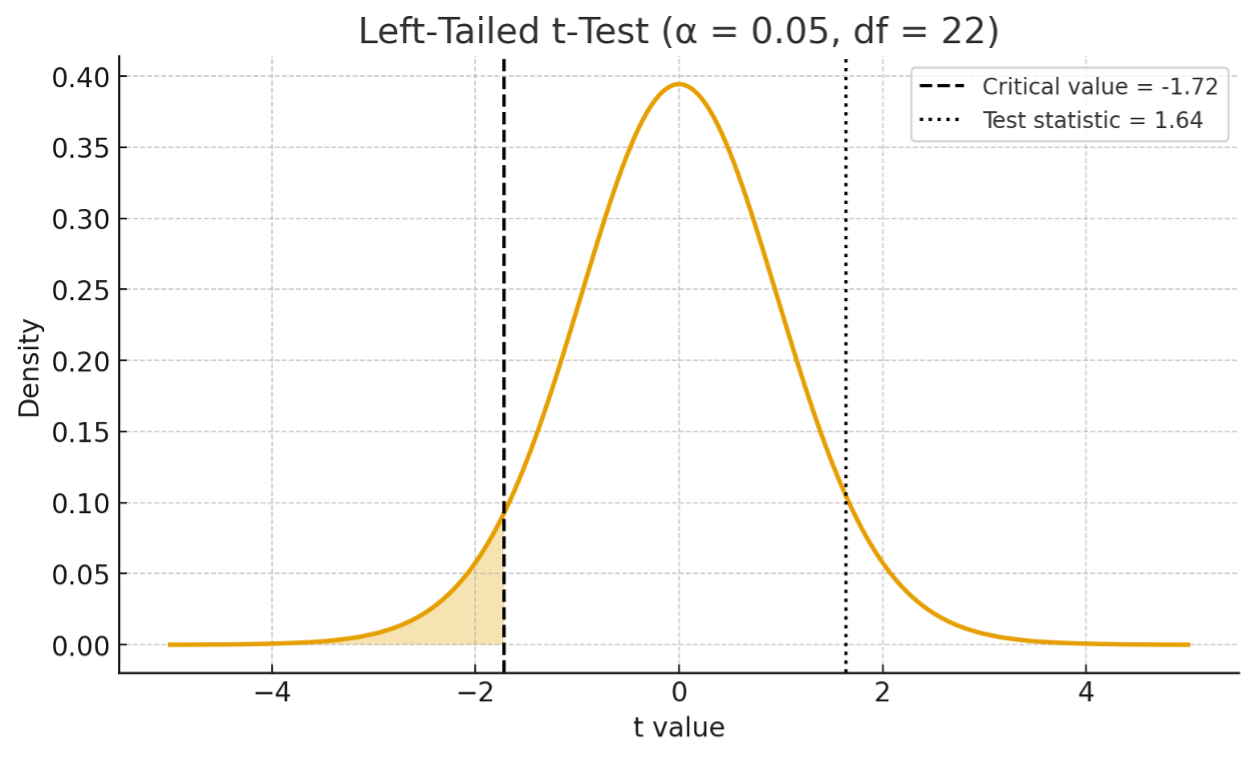
\includegraphics[width=0.95\textwidth,height=\textheight]{Fig/q1_b.png}

}

\end{figure}
\end{frame}

\begin{frame}{Exercise 1 (Cont'd)}
\protect\hypertarget{exercise-1-contd-4}{}
\begin{enumerate}
\setcounter{enumi}{2}
\item
  Test the claim that the correlation is different from zero using a 5\%
  level of significance. \vspace{-5pt}

  \pause

  \[
   \begin{aligned}
   H_0 &: \rho = 0 \\
   H_1 &: \rho \neq 0
   \end{aligned}
   \]

  \pause

  The significance level is \(\alpha=5\%\). To find the critical value
  for rejecting the null at this significance level, we look for the
  probability of \(0.05/2=0.025\) in the \textbf{Student's
  t-distribution} table with a degree of freedom \(df=n-2=24-2=22\). For
  a \textbf{two-tailed test}, we look for the value \(t\) such that the
  probability to its \textbf{left and right} is 0.025. From the table,
  we find that \(Pr(T>2.07)= 0.975\). Therefore, the critical value for
  a two-tailed test at the 5\% significance level is ±2.07. Since the
  t-test statistic (1.64) is between than the critical values (±2.07),
  we fail to reject the null hypothesis at a 5\% level of significance.
\end{enumerate}
\end{frame}

\begin{frame}{Exercise 1 (Cont'd)}
\protect\hypertarget{exercise-1-contd-5}{}
\pause

\vspace{15pt}

\begin{figure}

{\centering 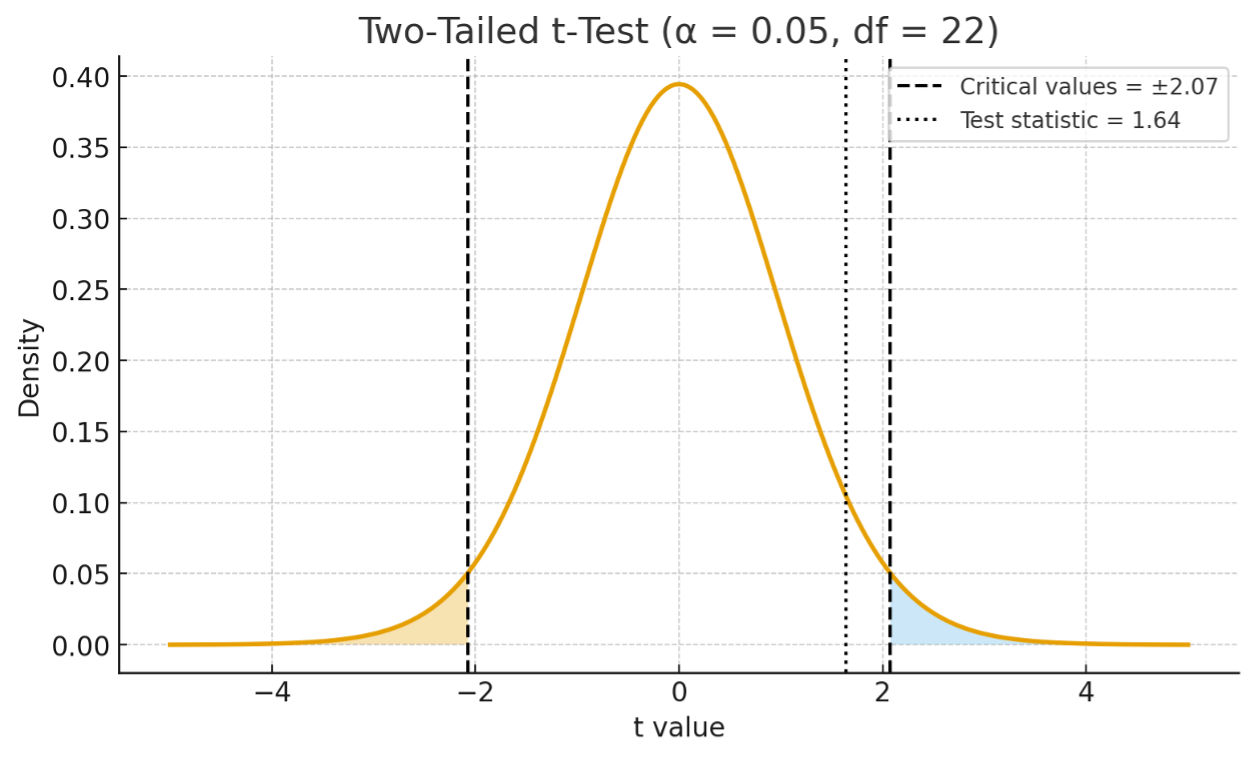
\includegraphics[width=0.95\textwidth,height=\textheight]{Fig/q1_c.png}

}

\end{figure}
\end{frame}

\begin{frame}{Exercise 2}
\protect\hypertarget{exercise-2}{}
\begin{table}[h!]
\centering
\begin{tabular}{cc}
\hline
Y & X \\
\hline
2   & 1 \\
4   & 2 \\
8   & 3 \\
16  & 4 \\
32  & 5 \\
64  & 6 \\
128 & 7 \\
\hline
\end{tabular}
\end{table}
\end{frame}

\begin{frame}{Exercise 2 (Cont'd)}
\protect\hypertarget{exercise-2-contd}{}
\begin{enumerate}
\item
  Estimate a regression of Y on X and interpret your results.

  \pause

  We have \(\hat{\beta}_1 = \frac{522}{28} \approx 18.64\). Therefore,
  we have \(\hat{\beta}_0 = 36.29 - 18.64 \times 4 = -38.29\). The
  estimated regression is then: \(Y = -38.29 + 18.64 \times X + Error\).
  \(\hat{\beta}_0\) suggests the predicted value of \(Y\) is -38.29 when
  \(X\) is zero and \(\hat{\beta}_1\) of 18.64 suggests an increase of
  one unit of \(X\) is associated with 18.64 unit increase in \(Y\).
\end{enumerate}
\end{frame}

\begin{frame}{Exercise 2 (Cont'd)}
\protect\hypertarget{exercise-2-contd-1}{}
\begin{enumerate}
\setcounter{enumi}{1}
\item
  Test if the slope coefficient is significantly different from zero at
  1\% level of significance. (The standard error for the slope
  coefficient is 4.55)

  \pause

  From (1), \(\hat{\beta}_1 = 18.64\), and \(SE(\hat{\beta}_1) = 4.55\):

  \pause

  \[
   \begin{aligned}
   H_0 &: \beta_1 = 0 \\
   H_1 &: \beta_1 \neq 0
   \end{aligned}
   \]

  \pause

  Next, we have the test statistic as follows

  \pause

  \[
   t = \frac{\hat{\beta_1} - 0}{SE(\hat{\beta_1})} = \frac{18.64 - 0}{4.55} \approx 4.1
   \]
\end{enumerate}
\end{frame}

\begin{frame}{Exercise 2 (Cont'd)}
\protect\hypertarget{exercise-2-contd-2}{}
\pause

The significance level is \(\alpha=1\%\). To find the critical value for
rejecting the null at this significance level, we look for the
probability of \(0.01/2=0.005\) in the \textbf{Student's t-distribution}
table with a degree of freedom \(df=n-2=7-2=5\). For a
\textbf{two-tailed test}, we look for the value t such that the
probability to its \textbf{left and right} is 0.005. From the table, we
find that \(Pr(T>4.03)= 0.995\). Therefore, the critical value for a
two-tailed test at the 5\% significance level is ±4.03. Since the t-test
statistic (4.1) is \emph{greater} than the critical values (4.03), we
reject the null hypothesis at a 5\% level of significance.
\end{frame}

\begin{frame}{Exercise 2 (Cont'd)}
\protect\hypertarget{exercise-2-contd-3}{}
\pause

\vspace{15pt}

\begin{figure}

{\centering 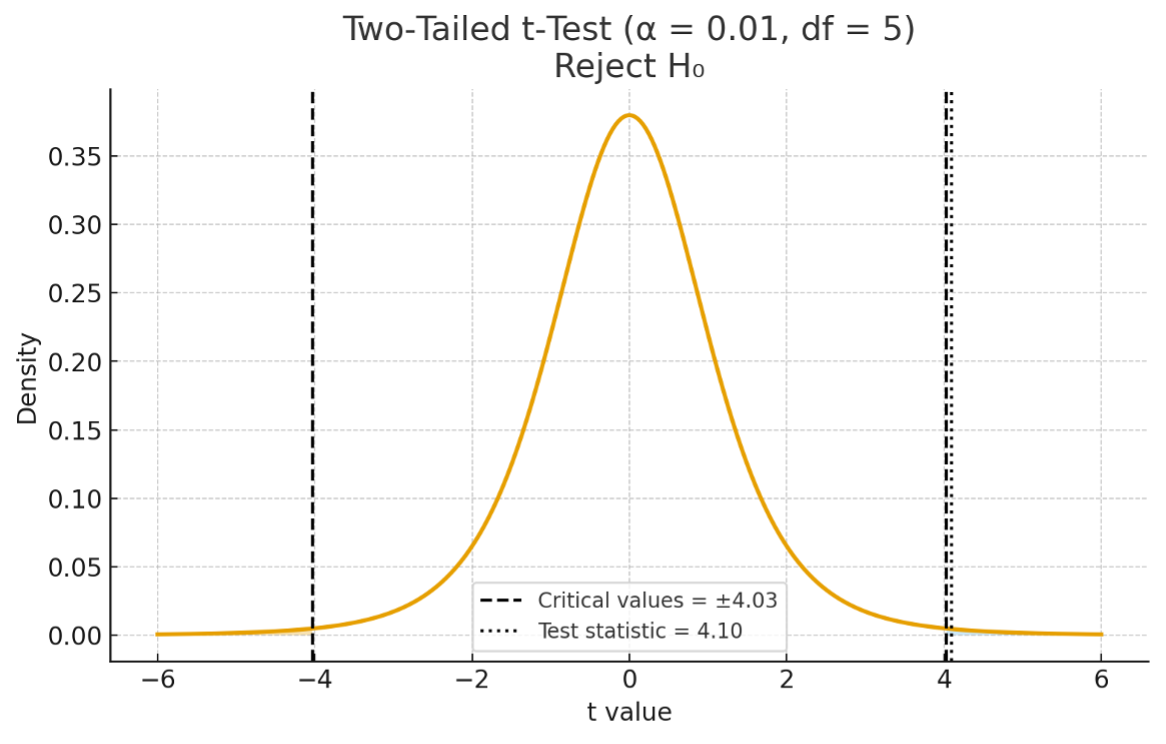
\includegraphics[width=0.95\textwidth,height=\textheight]{Fig/q2_b.png}

}

\end{figure}
\end{frame}

\begin{frame}{Exercise 2 (Cont'd)}
\protect\hypertarget{exercise-2-contd-4}{}
\begin{enumerate}
\setcounter{enumi}{2}
\item
  Compute the coefficient of determination and interpret your results.

  \pause

  The coefficient of determination for a simple linear regression can be
  computed as the square of the correlation coefficient. Therefore, we
  have: \vspace{-5pt}

  \pause

  \[
   R^2= \bigg(\frac{Cov(X,Y)}{S_X S_Y}\bigg)^2= \bigg(\frac{87}{2.16 \times 45.88}\bigg)^2=0.77.
   \]

  \pause

  This suggests the model explains 77\% of variation in Y.
\end{enumerate}
\end{frame}

\begin{frame}{Exercise 2 (Cont'd)}
\protect\hypertarget{exercise-2-contd-5}{}
\begin{enumerate}
\setcounter{enumi}{3}
\item
  Predict the value of Y when X is 3 and when X is 8.

  \pause

  When \(X=3\), we have \(Y= -38.29+18.64 \times 3=17.64\). Since
  \(X=8\) is out of the data range used to estimate the regression, we
  cannot predict the value of \(Y\) as this would lead to extrapolation.
\end{enumerate}
\end{frame}

\begin{frame}{Exercise 3}
\protect\hypertarget{exercise-3}{}
The cost of debt represents the required rate of return that firms must
offer to raise debt capital, where a lower cost implies more favourable
financing conditions. An analyst claims firms with more sales can assess
lower cost of debt. To investigate this, the analyst collects
cost-of-debt data for 15 firms, as shown in Table 1
\end{frame}

\begin{frame}{Exercise 3 (Cont'd)}
\protect\hypertarget{exercise-3-contd}{}
\begin{enumerate}
\item
  Estimate the regression of Cost of Debt on Sales and interpret the
  estimated coefficients.

  \pause

  We have \(\hat{\beta}_1 = \frac{-239.27}{427.73} \approx -0.56\).
  Therefore, we have \(\hat{\beta}_0 = 6.47-0.56 \times 7.47=10.64\).
  The estimated regression is then:
  \(Cost of Debt= 10.64-0.56 \times Sales+Error\). \(\hat{\beta}_0\) of
  10.64 suggests the predicted Cost of Debt is 10.64\% when Sales are
  zero and \(\hat{\beta}_1\) of -0.56 suggests an increase of one unit
  of Sales is associated with 0.56 unit decrease in Cost of Debt.
\end{enumerate}
\end{frame}

\begin{frame}{Exercise 3 (Cont'd)}
\protect\hypertarget{exercise-3-contd-1}{}
\begin{enumerate}
\setcounter{enumi}{1}
\item
  Using the reported standard error of the slope coefficient (0.10),
  test the analyst's claim at the 1\% level of significance.

  \pause

  From (1), \(\hat{\beta}_1 = -0.56\), and \(SE(\hat{\beta}_1) = 0.10\)

  \pause

  \[
   \begin{aligned}
   H_0 &: \beta_1 = 0 \\
   H_1 &: \beta_1 < 0 \\
   \end{aligned}
   \]

  \pause

  Next, we have the test statistic as follows

  \pause

  \[
   t = \frac{\hat{\beta}_1 - 0}{SE(\hat{\beta}_1)} = \frac{-0.56 - 0}{0.10} \approx -5.48
   \]
\end{enumerate}
\end{frame}

\begin{frame}{Exercise 3 (Cont'd)}
\protect\hypertarget{exercise-3-contd-2}{}
\pause

The significance level is \(\alpha=1\%\). To find the critical value for
rejecting the null at this significance level, we look for the
probability of 0.01 in the \textbf{Student's t-distribution} table with
a degree of freedom \(df=n-2=15-2=13\). For a \textbf{left-tailed test},
we look for the value t such that the probability to its \textbf{left}
is 0.01. From the table, we find that \(Pr(T>-2.65)= 0.99\). Therefore,
the critical value for a left-tailed test at the 5\% significance level
is -2.65. Since the t-test statistic (-5.48) is \emph{less} than the
critical values (-2.65), we reject the null hypothesis at a 1\% level of
significance.
\end{frame}

\begin{frame}{Exercise 3 (Cont'd)}
\protect\hypertarget{exercise-3-contd-3}{}
\pause

\vspace{15pt}

\begin{figure}

{\centering 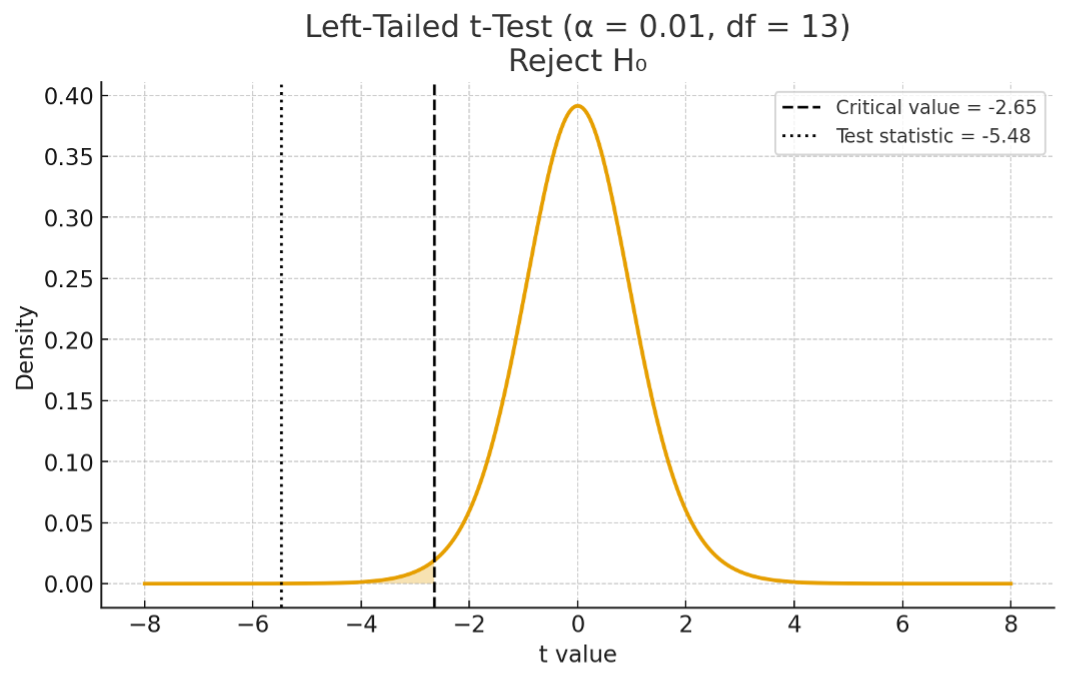
\includegraphics[width=0.95\textwidth,height=\textheight]{Fig/q3_b.png}

}

\end{figure}
\end{frame}

\begin{frame}{Exercise 3 (Cont'd)}
\protect\hypertarget{exercise-3-contd-4}{}
\begin{enumerate}
\setcounter{enumi}{2}
\item
  Compute the coefficient of determination (\(R^2\)) for the regression
  and interpret its meaning in context.

  \pause

  The coefficient of determination for a simple linear regression can be
  computed as the square of the correlation coefficient. Therefore, we
  have \vspace{-5pt}

  \pause

  \[
   R^2 = \bigg(\frac{Cov(X, Y)}{S_X S_Y} \bigg)^2 = \bigg(\frac{-17.09}{3.70 \times 5.53} \bigg)^2 = 0.70
   \]

  \pause

  This suggests the model explains 70\% of variation in Cost of Debt.
\end{enumerate}
\end{frame}

\begin{frame}{Exercise 3 (Cont'd)}
\protect\hypertarget{exercise-3-contd-5}{}
\begin{enumerate}
\setcounter{enumi}{3}
\item
  Suppose the true model includes another variable that affects the Cost
  of Debt and is also correlated with Sales, but this variable is
  omitted from the regression. Discuss how this omission would affect
  the estimated slope coefficient. No Calculations Required.

  \pause

  Omitting a variable that is correlated with Sales and affects Cost of
  Debt would lead to \textbf{omitted variable bias}. This would lead to
  a biased estimation of the coefficient for Sales.
\end{enumerate}
\end{frame}

\begin{frame}{Exercise 3 (Cont'd)}
\protect\hypertarget{exercise-3-contd-6}{}
\begin{enumerate}
\setcounter{enumi}{4}
\item
  If an additional explanatory variable is added to the regression and
  the \(R^2\) value increases, can we conclude that the new model is
  better? Answer Yes or No.~If your answer is No, explain why and
  describe the correct criterion for model comparison.

  \pause

  No as \(R^2\) can increase mechanically when we add additional
  variable into the model, regardless of whether the additional variable
  contains information or not. A better measurement would be to examine
  the adjusted \(R^2\) which accounts for degrees of freedom.
\end{enumerate}
\end{frame}

\begin{frame}{Exercise 4}
\protect\hypertarget{exercise-4}{}
A labour economist estimates the following multiple linear regression
model for hourly wage (in £) \vspace{-15pt}

\[
Wage=5.0+0.8 \times Schooling+0.3 \times Experience+2.5 \times Male+u 
\]

where:

\begin{itemize}
\item
  Schooling = years of education,
\item
  Experience = years of labour-market experience,
\item
  Male = 1 if the worker is male, 0 if female.
\end{itemize}

The regression is based on a sample of 100 workers. The reported \(R^2\)
is 0.78.
\end{frame}

\begin{frame}{Exercise 4 (Cont'd)}
\protect\hypertarget{exercise-4-contd}{}
\begin{enumerate}
\item
  Interpret each coefficient in the regression model.

  \pause

  The intercept of 5.0 suggests the predicted wage is £5 per hour for a
  female worker (Male = 0) with 0 years of schooling and 0 years of
  experience. Schooling (0.8) suggests each additional year of schooling
  is associated with an increase of £0.80 per hour in wage on average,
  holding \textbf{experience} and \textbf{gender} fixed. Experience
  (0.3) suggests each extra year of labour-market experience is
  associated with an increase of £0.30 per hour in wage on average,
  holding \textbf{schooling} and \textbf{gender} fixed. Male (2.5)
  suggests male workers earn £2.50 per hour more than otherwise similar
  female workers on average, holding \textbf{schooling} and
  \textbf{experience} fixed.
\end{enumerate}
\end{frame}

\begin{frame}{Exercise 4 (Cont'd)}
\protect\hypertarget{exercise-4-contd-1}{}
\begin{enumerate}
\setcounter{enumi}{1}
\item
  Compute the adjusted \(R^2\). Explain what \(R^2\) and adjusted
  \(R^2\) each measure, and which is more useful when comparing models.

  \pause

  We are given that \(R^2=0.78\), \(n=100\), and \(k=3\) \vspace{-15pt}

  \pause

  \[
   \begin{aligned}
   Adjusted\; R^2&=1-(1-R^2 )\frac{(n-1)}{(n-k-1)} \\ &=1-(1-0.78)\frac{(100-1)}{(100-3-1)}\approx0.773
   \end{aligned}
   \]
\end{enumerate}
\end{frame}

\begin{frame}{Exercise 4 (Cont'd)}
\protect\hypertarget{exercise-4-contd-2}{}
\pause

Therefore, the adjusted \(R^2\) is approximately 0.773. \(R^2=0.78\)
suggests about 78\% of the variation in wages in the sample is explained
by the linear relationship with schooling, experience, and gender.
Adjusted \(R^2=0.773\) is similar, but it penalises the model for
including more explanatory variables. It adjusts for degrees of freedom
so that adding a useless regressor does not artificially inflate the
goodness of fit. When comparing models with different numbers of
regressors, adjusted \(R^2\) is more useful, because it penalises
overfitting and only increases when a new variable improves the fit
``enough''.
\end{frame}

\begin{frame}{Exercise 4 (Cont'd)}
\protect\hypertarget{exercise-4-contd-3}{}
\begin{enumerate}
\setcounter{enumi}{2}
\item
  Suppose we re-estimate the model but omit Schooling from the
  regression. Discuss what is likely to happen to the estimated
  coefficients and why. \textbf{No Calculations Required}.

  \pause

  Schooling is almost certainly correlated with wage and likely
  correlated with experience and gender (e.g.~men and women may have
  different average schooling; more schooling might be linked to
  different career paths and thus experience). Leaving out an important,
  correlated variable leads to \textbf{omitted variable bias}. The new
  coefficients on \textbf{Experience} and \textbf{Male} will generally
  be biased and inconsistent: they will now partly pick up the effect of
  schooling, because the model is forcing them to explain variation that
  belongs to the omitted variable (i.e.~\textbf{Schooling}).
\end{enumerate}
\end{frame}



\end{document}
